% Chapter 2
\chapter{Piste n° 1} % Main chapter title
\label{Chapter2} % For referencing the chapter elsewhere, use \ref{Chapter2}
%----------------------------------------------------------------------------------------

\begin{description}
  \item[Version du Kernel :] 3.14
  \item[Code de travail :] imx219.c (fichier de la solution 2 sur le rapport du
  09/01/2017)
\end{description}

Suite à l'exploration des 3 pistes, nous avons choisi de nous
concentrer sur la solution n°2 puisque le driver se compile sans erreur. Cependant
il ne se charge pas dans le kernel.

\section{Erreur}
Constat : Le driver apparait à la commande lsmod mais est inutilisé.

 \begin{figure}[th]
   \centering
   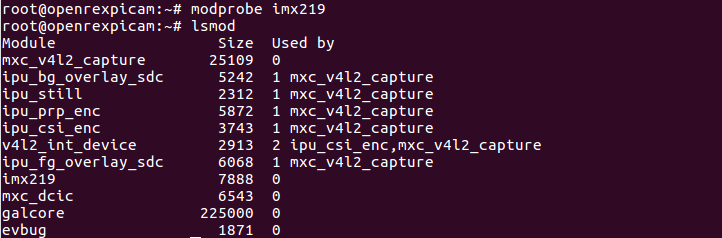
\includegraphics[width=1\linewidth]{chargement_driver.png}
   \decoRule
   \caption{Chargement du module}  \label{fig:Chargement-du-module}
\end{figure}

Après recherche d'indices pour le debug, on obtient le message d'erreur suivant:
\begin{figure}[th]
  \centering
  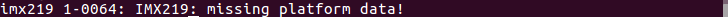
\includegraphics[width=1\linewidth]{errorplatform_dta.png}
  \decoRule
  \caption{Debug probe platform data}  \label{fig:Debug-probe-platform-data}
\end{figure}

Résultat de l'analyse :
l'erreur provient de la fonction probe du driver. La
sécurité testant le premier paramètre d'appel du driver s'est déclanchée. Le
paramètre est une structure contenant des informations sur les périphériques i2c.
Il y a donc un problème de compatibilité entre le driver imx219 et le gestionnaire i2c. Selon
l'avis de notre professeur de linux embarqué qui a appuyé nos recherches,
le driver en question utilise les interfaces de fonctionnement nommées
platform\_data, technologie remplacée progressivement depuis 2011 par le
device-tree et sa gestion des compatibilités.

\section{Solution}
Aujourd'hui mardi 16 janvier nous avons cherché à porter le driver vers
une compatibilité avec le device-tree.
\begin{description}
  \item[Ajout de la structure type of\_device\_id dans le driver]
  \begin{lstlisting}
  static const struct of_device_id imx219_of_match[] = {
    { .compatible = "sony,imx219", .data = 0 },
    {}
  };

  MODULE_DEVICE_TABLE(of, imx219_of_match);
  \end{lstlisting}

  \item[Completion de la structure de manipulation du driver]
  \begin{lstlisting}
  static struct i2c_driver imx219_i2c_driver = {
    .driver = {
      .name = "imx219",
      .of_match_table = of_match_ptr(imx219_of_match),
    },
    .probe		= imx219_probe,
    .remove	= imx219_remove,
    .id_table	= imx219_id,
  };
  \end{lstlisting}

  \item[Suppression de la sécuritée platform data]
  \begin{lstlisting}
    if (!ssdd) {
      dev_err(&client->dev, "IMX219: missing platform data!\n");
      return -EINVAL;
    }
    \end{lstlisting}
\end{description}

\section{Conclusion}
Une nouvelle erreur est apparue cependant les travaux qui concernent le
device tree ont fonctionné correctement car on peut remarquer au démarage
que le driver est chargé automatiquement.

\section{Erreur}
Au chargement de la nouvelle image nous obtenons l'erreur suivante:

\begin{figure}[th]
  \centering
  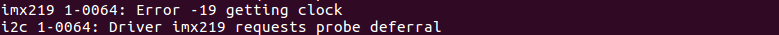
\includegraphics[width=1\linewidth]{errorclk.png}
  \decoRule
  \caption{Debug probe clk}  \label{fig:Debug-probe-clk}
\end{figure}

L'erreur est relative à la fonction getclk du driver qui est une sécurité comme la fonction supprimée précedement.
Elle confirme que nous avons des dificultés à communiquer avec l'i2c.

\section{Solution}
Notre strategie est de supprimer cette nouvelle fonction de securité, pour avoir plus
d'informations sur la façon dont le driver fonctionne.
\begin{description}
  \item[Suppression de la securité d'horloge]
    \begin{lstlisting}
	  if (IS_ERR(priv->clk)) {
		    dev_info(&client->dev, "Error %ld getting clock\n",
			  PTR_ERR(priv->clk));
		    return -EPROBE_DEFER;
	  }
    \end{lstlisting}
\section{Conclusion}
Le driver est maintenant chargé "correctement" par le kernel.

\begin{figure}[th]
  \centering
  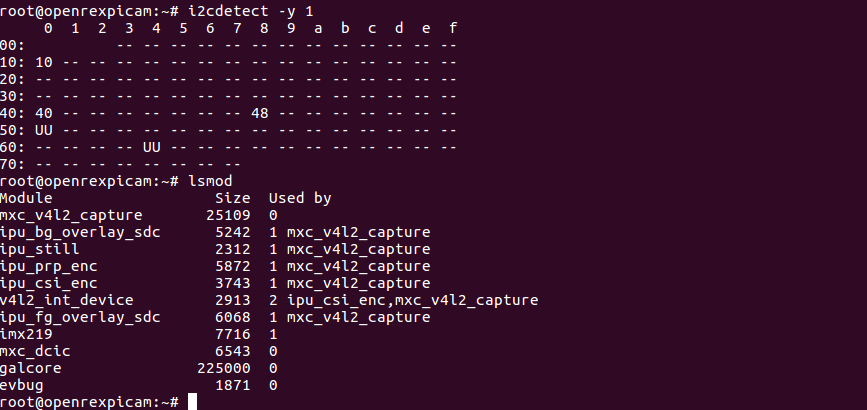
\includegraphics[width=1\linewidth]{lsmodeti2cdetect.png}
  \decoRule
  \caption{Chargement du module}  \label{fig:chargement}
\end{figure}
\end{description}

  On peut voir que le driver imx219 est chargé par l'i2c et
  qu'il est utilisé par un autre module. Nous ne sommes toujours pas en mesure
  de nous en servir car il nous manque des informations sur son fonctinnement.
  De plus de nouvelles erreurs apparaissent au chargement du driver.

\clearpage

  \section{Erreur}
  Au chargement du driver nous obtenons le message de debug kernel suivant:

  \begin{figure}[th]
    \centering
    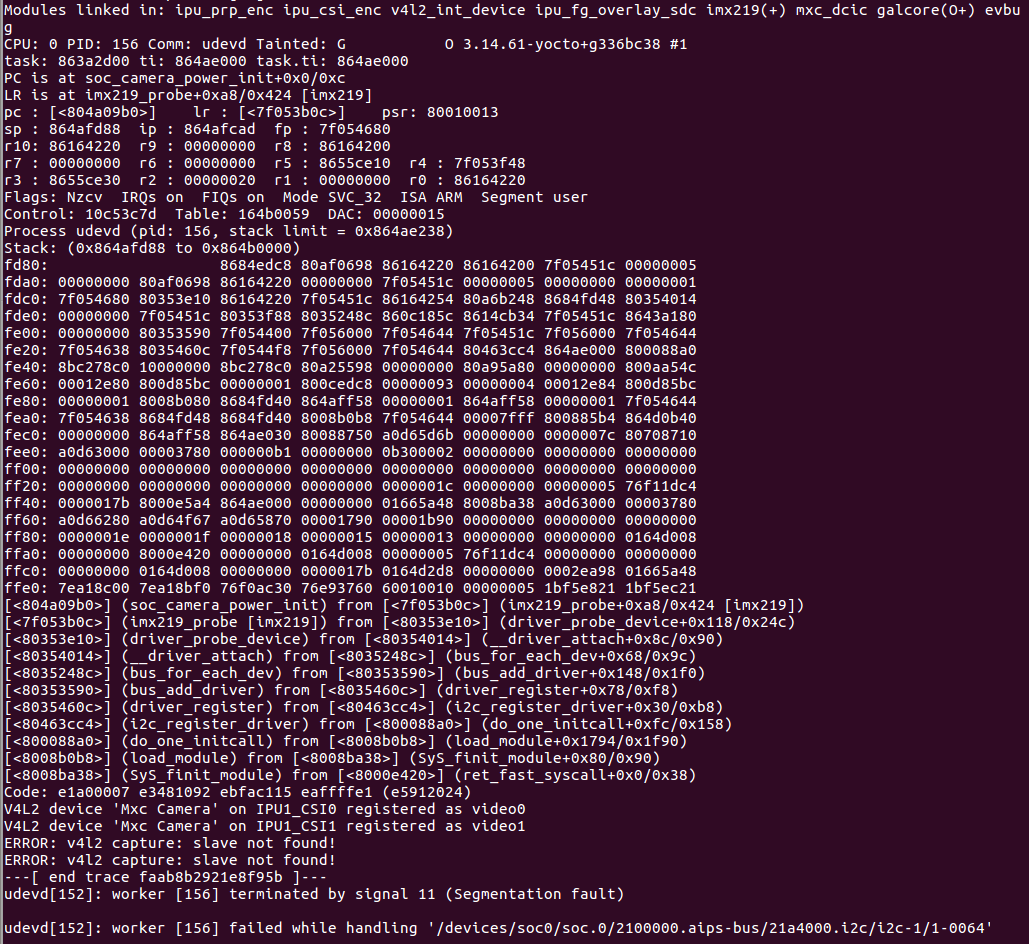
\includegraphics[width=1\linewidth]{debugdmesg.png}
    \decoRule
    \caption{Dmsg}  \label{fig:dmsg}
  \end{figure}

  \section{Reste à faire}

  \begin{itemize}
  \item[-] Determiner la cause du segmentation fault.
  \item[-] Savoir comment récuperer le flux video.
  \end{itemize}
    %----------------------------------------------------------------------------------------
